\documentclass[11pt]{article}
\usepackage[margin=1in]{geometry}
\usepackage{tikz}
\usepackage{array}
\usepackage{amsmath}
\begin{document}
\section*{Cantilever beam under pure torque}
A fixed-free beam is subjected to an end torque $T=1000$ Nm about the beam axis. The material and section data are $E=2.0690e+11$ Pa, $\nu=0.29$, $G=8.0194e+10$ Pa, $I_z=1$ m$^4$, $J=1$ m$^4$, and $L=10$ m.

\subsection*{Configuration}
\begin{center}
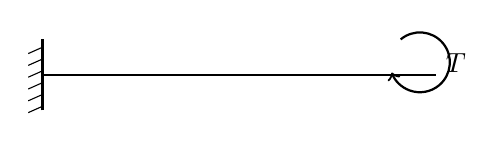
\begin{tikzpicture}[scale=1.0]
\draw[thick] (0,0)--(5,0);\draw[very thick] (0,-0.45)--(0,0.45);\foreach \y in {-0.4,-0.25,...,0.4}{\draw (-0.18,\y-0.08)--(0,\y);}\draw[->,thick] (4.55,0.45) arc[start angle=130,end angle=-160,radius=0.38];\node[right] at (5,0.15) {$T$};
\end{tikzpicture}
\end{center}

\subsection*{Analytical Reference}
$\theta_x(L)=TL/(GJ)$.

\subsection*{Numerical Comparison}
\begin{center}
\begin{tabular}{|>{\raggedright\arraybackslash}p{0.18\linewidth}|r|r|r|r|r|}
\hline
Quantity & Analytical & C++ & Python & Python vs. analytical & Python vs. C++ \\
\hline
$\theta_x(L)$ & 1.24697922e-07 & 1.24697920e-07 & 1.24697920e-07 & 1.364e-06\% & 0.000e+00\% \\
\hline
\end{tabular}
\end{center}

\subsection*{Evaluation}
The Python and C++ results are numerically identical to the precision written in the VTK files for the selected critical quantities. The remaining discrepancy with the analytical expression is governed by the finite element discretization and by the equivalent nodal loading representation where applicable.
\end{document}
